\section{Rachunek \(\lambda\) z typami prostymi}

%System \(\lambda_{\to}\) w stylu Churcha to zbiór typów \(\mathrm{T}\),
%zbiór pseudotermów \(\Lambda_{\mathrm{T}}\), rodzina otoczeń typowych,
%relacja \(\beta\)-kontrakcji \(\to_{\beta}\) i relacja przypisania typu \(\vdash\).

\subsection{Typy proste}\label{ssec:typy-proste}
Niech \(\mathrm{U}\) będzie przeliczalnie nieskończonym zbiorem zmiennych przedmiotowych \(p,\ q,\ \dots\ \) (być może indeksowanych liczbami naturalnymi), które będziemy nazywali \emph{zmiennymi typowymi}.\begin{definicja}\label{def:typy-proste}(Typy proste)\\
\emph{Typami prostymi} będziemy określali najmniejszy w sensie mnogościowym zbiór wyrażeń taki, że:
\begin{enumerate}[label=T\arabic*.]
  \item Jeśli \(p\) jest zmienną typową, to \(p\) jest typem prostym.
  \item Jeśli \(\tau\) i \(\sigma\) są typami prostymi, to \(\left(\tau\to\sigma\right)\) jest typem prostym.
\end{enumerate}
\end{definicja}

Typy proste zbudowane tylko wedle reguły T1 nazywamy typami \emph{atomowymi}, zaś wyrażenia zbudowe wedle reguły T2 -- typami \emph{funkcyjnymi}. Zbiór typów prostych określony w myśl powyższej definicji będziemy oznaczali przez \(\mathbf{T_\to}\).

Późniejsze litery alfabetu greckiego, tj. \(\sigma,\, \tau,\, \rho,\ \dots\) będą służyły nam za zmienne metasyntaktyczne do oznaczania typów prostych. Dla lepszej czytelności będziemy pomijali najbardziej zewnętrzne nawiasy. Konstruktor typu \(\to\) jest prawostronnie łączny, co oznacza, że typy \(\tau\to\sigma\to\theta\) oraz \(\tau\to(\sigma\to\theta)\) będziemy uznawali za tożsame.

Typy proste ujęte Definicją \ref{def:typy-proste} mają strukturę drzewa binarnego. Wysokość takiego drzewa będziemy nazywali \emph{stopniem} typu. Precyzyjnie ujmuje to pojęcie poniższa definicja.
\begin{definicja}\label{def:stopien-typu}(Stopień typu)\\
  Stopniem typu nazywamy funkcję 
  \begin{align*}
    \delta(p) &= 0,\\
    \delta(\tau\to\sigma)&=1 + \max\left(\delta(\tau),\ \delta(\sigma)\right).
  \end{align*}
\end{definicja}

\subsection{Pseudotermy}
  Niech \(\mathrm{V}\) będzie przeliczalnie nieskończonym zbiorem zmiennych przedmiotowych \(x,\ y,\ \dots\ \) (indeksowanych być może liczbami naturalnymi). Elementy takiego zbioru będziemy nazywali \emph{\(\lambda\)-zmiennymi}.
\begin{definicja}(Pseudo-pretermy)\\
  \emph{Pseudo-pretermami} będziemy nazywali najmniejszy (w sensie mnogościowym) zbiór \(\mathbf{\Lambda}^{-}_{\mathrm{T}}\) taki, że:

\begin{enumerate}[label=P\arabic*.]
    \item Jeśli \(x\in \mathrm{V}\), to \(x\in\mathbf{\Lambda}^{-}_{\mathrm{T}}\).
    \item Jeśli \(M\in\mathbf{\Lambda}^{-}_{\mathrm{T}}\) i \(N\in\mathbf{\Lambda}^{-}_{\mathrm{T}}\), to \((MN)\in\mathbf{\Lambda}^{-}_{\mathrm{T}}\).
    \item Dla dowolnych \(x\in \mathrm{V}\), \(\sigma\in\mathbf{T}_\to\), \(M\in\mathbf{\Lambda}^{-}_{\mathrm{T}}\) mamy, że \((\lambda x^{\sigma}.\,M)\in \mathbf{\Lambda}^{-}_{\mathrm{T}}\).
  \end{enumerate}
\end{definicja}
  Wyrażenia postaci P2 nazywamy \emph{aplikacjami} \(M\) do \(N\), zaś wyrażenia postaci P3 -- \(\lambda\)-abstrakcjami, gdzie o wszystkich podtermach termu \(M\) mówi się, że są w \emph{zasięgu} \(\lambda\)-abstraktora, zaś o \(\lambda\)-zmiennej \(x\) mówi się, że jest \emph{związana}.

  Za zmienne metasyntaktyczne obieramy duże litery alfabetu łacińskiego \(M,\ N,\ \dots\ \) Podobnie jak w podrozdziale \ref{ssec:typy-proste} stosujemy konwencję o opuszczaniu najbardziej zewnętrznych nawiasów. Aplikacja termów jest łączna lewostronnie, co oznacza, że będziemy utożsamiali wyrażenia \(MNP\) oraz \((MN)P\).

\begin{definicja}(Zmienne wolne)
  \item Dla pseudo-pretermu \(M\) określamy zbiór \emph{termów wolnych} \(\mathrm{FV}\) w nastepujący sposób:
    \begin{align*}
      \mathrm{FV}(x) &= \{x\}\\
      \mathrm{FV}(\lambda x^\sigma .\, P)  &= \mathrm{FV}(P)\setminus\{x\}\\
      \mathrm{FV}(P Q) &= \mathrm{FV}(P)\cup\mathrm{FV}(Q)
    \end{align*}
Jesli \(\mathrm{FV}(M)=\emptyset\), to mówimy, że \(M\) jest \emph{zamknięty}. 
\end{definicja}
%  \item Podstawieniem pseudotermu \(N\) za \(\lambda\)-zmienną \(x\) w pseudotermie \(M\), symbolicznie \(M[x/N]\), nazywamy przekształcenie pseudotermu zadane następującymi warunkami:
%    \begin{enumerate}[label=({\alph*})]
%    \item Podstawienie jest poprawne wtedy i tylko wtedy, gdy żadne wolne wystąpienie \(\lambda\)-zmiennej \(x\) w pseudotermie \(M\) nie występuje w podtermie \(M\) postaci \(\lambda y.\, L\), gdzie \(y\in\mathrm{FV}(N)\).
%    \item
%      \begin{align*}
%        x[x/N] &= N,&\\
%        y[x/N] &= y,\ &\text{o ile}\ x\neq y,&\\
%        (PQ)[x/N] &= P[x/N]\,Q[x/N],&\\
%        (\lambda x.\,P)[x/N] &= \lambda x.\,P,&\\
%        (\lambda y.\,P)[x/N] &= \lambda y.\,P [x/N],\ &\text{o ile}\ x\neq y.
%      \end{align*}
%    \end{enumerate}

\begin{definicja}(Podstawienie)\\
\emph{Podstawieniem} \([x/N]\) pseudo-pretermu \(N\) za \(\lambda\)-zmienną \(x\) w \(M\) nazwamy zdefiniowane następująco przekształcenie:
  \begin{align*}
    x[x/N] &= N,\\
    y[x/N] &= y,\ &\text{o ile}\ x\neq y,\\
    (PQ)[x/N] &= P[x/N]\,Q[x/N],\\
    (\lambda y^\sigma.\, P)[x/N] &= \lambda y^\sigma .\,P[x/N],\ &\text{gdzie}\ x\neq y\ \text{i}\ y\not\in \mathrm{FV}(N).\\
  \end{align*}
\end{definicja}

\noindent Zachodzą następujące fakty:
    \begin{fakt}
      \begin{enumerate}[label=({\alph*})]
        \item Jeśli \(x\not\in\mathrm{FV}(M)\), to \(M[x/N]\) jest poprawnym podstawieniem i \(M[x/N]=M\).
        \item Jeśli \(M[x/N]\) jest poprawnym podstawieniem, to \(y\in\mathrm{FV}(M[x/N]\) wtw, gdy albo \(y\in\mathrm{FV}(M)\)
          i \(x\neq y\), albo \(y\in \mathrm{FV}(N)\) i \(x\in \mathrm{FV}(M)\). 
        \item Podstawienie \(M[x/x]\) jest poprawne i \(M[x/x]=M\).
        \item Jeśli \(M[x/y]\) jest poprawnym podstawieniem, to \(M[x/y]\) ma tę samą długość, co \(M\).
      \end{enumerate}
    \end{fakt}
    \begin{fakt}
      Powiedzmy, że \(M[x/N]\) jest poprawnym podstawieniem i \(N[y/L]\) i \(M[x/N][y/L]\) są poprawnymi podstawieniami, gdzie
      \(x\neq y\). Jeśli \(x\not\in \mathrm{FV}(L)\) lub \(y\not\in\mathrm{FV}(M)\), to \(M[y/L]\) i \( M[y/L]\left[x/N[y/L]\right] \) jest poprawnym podstawieniem oraz
      \[
        M[x/N][y/L]=M[y/L][x/N[y/L]].
      \]
    \end{fakt}

    \begin{fakt}
      Jesli \(M[x/y]\) jest poprawnym postawieniem i \(y\not\in\mathrm{FV}(M)\), to \(M[x/y][y/x]\) jest poprawnym podstawieniem oraz
      \(M[x/y][y/x]=M\).
    \end{fakt}
    
  \begin{definicja}(\(\alpha\)-konwersja)\\
    \(\alpha\)-konwersją nazywamy najmniejszą (w sensie mnogościowym) zwrotną i przechodnią relację binarną \(=_\alpha\) określoną na zbiorze pseudotermów \(\mathbf{\Lambda}^{-}_{\mathrm{T}}\) spełniającą poniższe warunki:
    \begin{enumerate}[label=({\alph*})]
      \item Jeśli \(y\not\in \mathrm{FV}(M)\) i \(M[x/y]\) jest poprawnym podstawieniem, to \(\lambda x.\, M  =_\alpha \lambda y.\, M[x/y]\).
      \item Jeśli \(M=_\alpha N\), to dla każdej \(\lambda\)-zmiennej \(x\) mamy \(\lambda x.\, M =_\alpha \lambda x.\,N\).
      \item Jeśli \(M=_\alpha N\), to \(M Z=_\alpha N Z\).
      \item Jeśli \(M=_\alpha N\), to \(ZM =_\alpha ZN\).
    \end{enumerate}
  \end{definicja}

\noindent Bez dowodu podajemy następujące twierdzenia:
    \begin{fakt}
      Relacja \(=_{\alpha}\) jest symetryczna.
    \end{fakt}
    \begin{fakt}
      \(=_{\alpha}\) jest relacją równoważności.
    \end{fakt}
    \begin{fakt}
      Jeśli \(M=_\alpha N\), to \(\mathrm{FV}(M)=\mathrm{FV}(N)\).
    \end{fakt}

Dysponując powyższymi rozstrzygnięciami otrzymujemy wygodne utożsamienie pseudo-pretermów,
które różnią się między sobą tylko zmiennymi związanymi.

\begin{definicja}(Pseudotermy)\\
  Klasy abstrakcji relacji \(\alpha\)-konwersji nazywamy \emph{pseudotermami}. Zbiór wszystkich pseudotermów oznaczamy następująco:
\[
  \mathbf{\Lambda}_{\mathrm{T}}=\left\{[M]_\alpha\:|\: M\in\mathbf{\Lambda}^{-}_\mathrm{T}\right\}
\]
\end{definicja}
Nadużywając notacji będziemy odnosili się do pseudotermów tylko przez ich reprezentantów.
\subsection{Typowalność} 
%\item
%  \emph{Pseudo-pretermami} nazywamy język \(\Lambda_{\mathrm{T}}\) generowany przez
%gramatykę 
%\[
%  \Lambda^{-}_{\mathrm{T}} := \ \mathrm{V}\ | \ \left (\lambda V^{\mathrm{T}} . \Lambda^{-}_{\mathrm{T}}\right) \ | \ \left (\Lambda^{-}_{\mathrm{T}}\Lambda^{-}_{\mathrm{T}}\right)
%\]
%    gdzie V to przeliczalny zbiór \(\lambda\)-zmiennych \(x, y, \dots\)
    
%    W języku podmiotowym będziemy używali późniejszych liter alfabetu łacińskiego pisanych kursywą (\(M,\, N,\, O,\, \dots\)) oznaczając pseudotermy.

\begin{definicja}(Kontekst)\\
  \emph{Kontekstem} nazywamy skończoną funkcję częściową \(\Gamma:\:\mathrm{V}\longrightarrow\mathbf{T_\to}\), czyli zbiór par postaci \(\Gamma=\{x_1^{\tau_1},\,\dots,\,x_n^{\tau_n}\},\ \text{gdzie}\ (x_i^{\tau_i})=(x_i,\, \tau_i)\ \text{oraz}\ x_i \neq x_j\ \text{dla}\ i\neq j\). Zbiór 
  \[\mathrm{dom}(\Gamma) = \left\{x\in \mathrm{V}\,|\,\exists\tau(x^\tau\in\Gamma)\right\}\]
  nazywamy \emph{dziedziną} kontekstu \(\Gamma\), zaś 
  \[\mathrm{rg}(\Gamma)=\left\{\tau\in\mathbf{T}_\to\,|\,\exists x(x^\tau\in\Gamma)\right\}\]
  -- \emph{zakresem} kontekstu \(\Gamma\).
  Piszemy:
  \begin{itemize}
    \item \(x_{1}^{\tau_1},\,x_{2}^{\tau_2}\) zamiast \(\{x_{1}^{\tau_1},\, x_{2}^{\tau_2}\}\), o ile \(x_{1}^{\tau_1}\) i \(x_{2}^{\tau_2}\) są różne,
    \item \(\Gamma,\, x^\varphi\) zamiast \(\Gamma\cup \{x^\varphi\}\), o ile \(x^\varphi\not\in \Gamma\),
    \item \(\Gamma,\, \Delta\) zamiast \(\Gamma\cup \Delta\), o ile \(\Gamma\cap\Delta=\emptyset\).
  \end{itemize}
\end{definicja}

Okreslimy teraz system przypisywania typów do pseudotermów w stylu dedukcji naturalnej. \emph{Sekwentami} w tym systemie będziemy nazywali wyrażenia postaci \(\Gamma\vdash M^{\sigma}\), gdzie \(M\in\mathbf{\Lambda}_{\mathrm{T}},\ \sigma\in\mathbf{T_\to}\), zaś \(\Gamma\) jest pewnym kontekstem. 

Wprowadzamy następujące reguły dowodzenia:
    \begin{center}
    \begin{tabular}{ ccc}
      {\begin{prooftree}
        \Hypo{}
        \Infer1[(Var)]{\Gamma, x^\tau\vdash x^\tau}
      \end{prooftree}},
      &
      {\begin{prooftree}
        \Hypo{ \Gamma, x^{\varphi} \vdash M^{\psi} }
        \Infer1[(Abs)]{\Gamma \vdash (\lambda\, x^{\varphi}.\, M)^{\varphi\to\psi}}
      \end{prooftree}},
      &
      {\begin{prooftree}
        \Hypo{\Gamma \vdash M^{\varphi \to \psi}} \Hypo{ \Gamma \vdash N^{\varphi}}
        \Infer2[(App)]{\Gamma \vdash (MN)^{\psi}}
      \end{prooftree}}.
      \end{tabular}
    \end{center}

\begin{definicja}(Typowalność)\\
  Mówimy, że pseudoterm \(M\) jest typu \(\sigma\) w kontekście \(\Gamma\) (jest \emph{typowalny}), jeśli istnieje skończone drzewo sekwentów spełniające poniższe warunki:
  \begin{enumerate}
      \item W korzeniu drzewa znajduje się sekwent \(\Gamma \vdash M^\sigma\).
      \item Liście są \emph{aksjomatami}, tj. sekwentami postaci \(\Gamma, x^\sigma \vdash x^\sigma\).
      \item Każdego rodzica można otrzymać z jego dzieci przez zastosowanie którejś z reguł wyprowadzania nowych sekwentów.
  \end{enumerate}
  Tak określone drzewo będziemy nazywali \emph{wyprowadzeniem} typu.
\end{definicja}
 \begin{definicja}\label{def:lambda-term}(\(\lambda\)-termy)\\ 
   Wszystkie typowalne pseudotermy w pewnym kontekście \(\Gamma\) nazywamy \emph{\(\lambda\)-termami} (z typami prostymi w  kontekście \(\Gamma\)).
  \begin{uwaga*}
    \(\lambda\)-term w kontekście \(\Gamma_1\) może nie być typowalny w innym kontekście \(\Gamma_2\).   
  \end{uwaga*}
\end{definicja}
Mówiąc o \(\lambda\)-termach i nie podając żadnego związanego z nimi kontekstu \(\Gamma\) będziemy implicite zakładali, że istnieje pewien kontekst w którym są one typowalne. Zakładamy również, że ustalone są typy dla wszystkich \(\lambda\)-zmiennych. Typ dowolnego \(\lambda\)-termu będziemy w ramach konwencji notowali używając górnego indeksu. Dla przykładu, \(\lambda\)-term \(\left(M^{\sigma\to\tau}N^\sigma\right)^\tau\) jest w pewnym kontekście \(\Gamma\) typu \(\tau\). 

   Przez \emph{stopień} \(\lambda\)-termu \(M^\sigma\) będziemy mieli na myśli stopień typu \(\sigma\). Nadużywając notacji będziemy pisali
   \[
     \delta(M^\sigma) = \delta(\sigma),
   \]
   gdzie \(\delta\) występująca po prawej stronie powyższej równości to funkcja określona w myśl Definicji \ref{def:stopien-typu}.


  \begin{fakt}
    Jesli \(\Gamma\vdash M^\sigma\) oraz \(\Gamma\vdash M^\tau\), to \(\sigma=\tau\).
  \end{fakt}
\subsection{Redukcja}
\begin{definicja}(Zgodność)\\
  Relację \(\mathrm{R}\) na zbiorze termów \(\mathbf{\Lambda}_{\mathrm{T}}\) nazywamy \emph{zgodną}, jeśli dla \(M,\,N,\,Z\in\mathbf{\Lambda}_{\mathrm{T}}\) spełnia ona następujące warunki:
  \begin{enumerate}[label=\roman*)]
    \item Jeśli \(M\mathrm{R} N\), to \((\lambda x^\sigma.\,M)\, \mathrm{R}\, (\lambda x^\sigma.\, N)\) dla dowolnych \(x\in \mathrm{V}\) i \(\sigma\in \mathbf{T_\to}\).
    \item Jeśli \(M\mathrm{R} N\), to \((MZ)\,\mathrm{R}\, (NZ)\).
    \item Jeśli \(M\mathrm{R} N\), to \((ZM)\,\mathrm{R}\, (ZN)\).
  \end{enumerate}
Przy powyższych ustaleniach \emph{kongruencją} będziemy nazywali każdą zgodną relację równowazności na \(\mathbf{\Lambda}_{\mathrm{T}}\), zaś \emph{redukcją} – każdą zgodną, zwrotną i przechodnią relację na \(\mathbf{\Lambda}_{\mathrm{T}}\).
\end{definicja}

\begin{definicja}(\(\beta\)-redukcja)\\
  \(\beta\)-redukcją nazywamy najmniejsza w sensie mnogościowym \emph{zgodną} relację binarną \(\longrightarrow_{\beta}\) określoną zbiorze na pseudotermów \(\mathbf{\Lambda}_{\mathrm{T}}\) za pomocą podstawienia
  \[
    (\lambda x^\sigma.\,P)Q \longrightarrow_{\beta} P[x/Q].
  \]
  
  \noindent \emph{\(\beta\)-redeksami} bedziemy nazywali wyrażenia postaci \((\lambda x^\sigma.\, M)N\), zaś rezultat ich \(\beta\)-redukcji w postaci termu \(M[x/N]\) -- \emph{\(\beta\)-reduktem}.
\end{definicja}
\noindent Określamy następujące relacje:
\begin{enumerate}[label=B\arabic*.]
\item    \(\longrightarrow^{+}_{\beta}\) jest przechodnim domknięciem relacji \(\longrightarrow_{\beta}\) w zbiorze pseudotermów \(\mathbf{\Lambda}_{\mathrm{T}}\).

\item    \(\longrightarrow^{*}_{\beta}\) jest domknięciem przechodnio-zwrotnim w \(\mathbf{\Lambda}_{\mathrm{T}}\) relacji \(\longrightarrow_{\beta}\), a zatem jest \emph{redukcją}. 

\item    \(=_{\beta}\) jest najmniejszą relację równowazności zawierającą relację \(\longrightarrow_{\beta}\), (czyli \emph{kongruencją}).
\end{enumerate}

\begin{definicja}\label{def:postac-normalna}(Postać normalna)\\
  Powiemy, że \(\lambda\)-term \(M\) jest w \emph{postaci normalnej}, jeśli żadna z jego podformuł nie jest \(\beta\)-redeksem. Przez \(\mathrm{NF}_{\beta}\) będziemy oznaczali zbiór wszystkich \(\lambda\)-termów w postaci normalnej.
\end{definicja}    

Zachodzą następujące fakty:
\begin{fakt}
\(M\) \emph{ma postać normalną}, jeśli \(M=_{\beta}N\) dla pewnego \(N\), który jest w postaci normalnej.
\end{fakt}
\begin{fakt}
  Jeśli \(\Gamma\vdash M^\sigma\) i \(M\longrightarrow^{*}_{\beta}N\), to
  \(\Gamma\vdash N^\sigma\).
\end{fakt}
  
  \begin{definicja}(\(\eta\)-redukcja)\\
\(\eta\)-redukcją nazywamy najmniejszą (w sensie mnogościowym) \emph{zgodną} relację w \(\mathbf{\Lambda}_{\mathrm{T}}\) taką, że
  \[
    \lambda x^\sigma.\, Mx\longrightarrow_{\eta} M,
  \]
    o ile \(x\not\in \mathrm{FV}(M)\).
  \end{definicja}

  \begin{fakt}
    Jeśli \(\Gamma\vdash M^\sigma\) i \(M\longrightarrow^{*}_{\eta}N\), to
    \(\Gamma\vdash N^\sigma\).
  \end{fakt}

\subsection{Normalizacja}
\noindent Powiemy, że \(\lambda\)-term \(M\) ma własność:
\begin{easylist}
  & \emph{(słabej) normalizacji} (symbolicznie: \(M\in\mathrm{WN_{\beta}}\)) wtedy i tylko wtedy, gdy istnieje ciąg \(\beta\)-redukcji rozpoczynający się od \(M\) i kończący się termem w postaci normalnej \(N\). 
  &  \emph{silnej normalizacji} (symbolicznie: \(M\in\mathrm{SN_{\beta}}\)), jeśli wszystkie ciągi \(\beta\)-redukcji rozpoczynające się od \(M\) są skończone.
\end{easylist}
\noindent Z powyższego określenia  widzimy, że własność \(\mathrm{SN}_{\beta}\) pociąga za sobą własność \(\mathrm{WN}_{\beta}\).

\begin{definicja}(Strategia redukcji)\\
\emph{Strategią redukcji} nazywamy odwzorowanie \(F:\:\mathbf{\Lambda}_{\mathrm{T}}\longrightarrow\mathbf{\Lambda}_{\mathrm{T}}\) takie, że \(F(M)=M\), gdy \(M\) jest w postaci normalnej i \(M\to_{\beta}F(M)\) w przeciwnym wypadku. Mówimy, że strategia \(F\) jest \emph{normalizująca}, jeśli dla każdego \(M\in \mathrm{WN_\beta}\) istnieje \(i\in\mathbb{N}\) takie, że \(F^i (M)\) jest w postaci normalnej.
\end{definicja}

\begin{twierdzenie}(\emph{Własność \(\mathrm{WN}_{\beta}\)}) Wszystkie \(\lambda\)-termy mają postać normalną.
\end{twierdzenie}
\begin{dowod}
  Pokażemy, że dla dowolnego \(\lambda\)-termu \(M\) istnieje normalizująca strategia redukcji. 

  Przypuśćmy, że \(M\) nie jest w postaci normalnej. Oznaczmy przez \(\delta_M\) maksymalny stopień redeksów występujących w \(M\). Ponieważ wiele redeksów w \(M\) może mieć ten sam stopień \(\delta_M\), przez \(n_M\) oznaczmy liczbę ich wystąpień. 

  Niech \(\Delta\) będzie \(\beta\)-redeksem stopnia \(\delta_M\) położonym w \(M\) najbardziej na prawo i niech \(M'\) będzie \(\beta\)-reduktem otrzymanym przez zredukowanie \(\Delta\). Zauważmy, że \(n_M < n_{M'}\), gdyż \(\Delta\) nie wystepuje już w \(M'\), zaś \(\beta\)-redukcja \(\Delta\) może prowadzić do powstania redeksów tylko mniejszego stopnia. Istotnie, ilość redeksów w \(M\) może zwiększyć się tylko na jeden z poniższych sposobów: 
  \begin{enumerate}[label=\roman*)]
    \item powstanie nie występujących wcześniej redeksów.
    \item powielenie już istniejących redeksów.
  \end{enumerate}

  \begin{figure}[htb]
  \centering
  \begin{subfigure}{0.55\textwidth}
    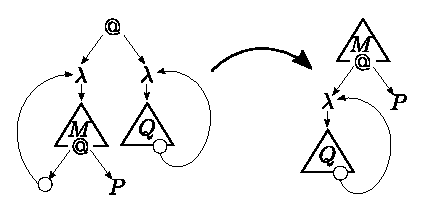
\includegraphics[width=1\linewidth]{../reduction1}
    \caption{Redukcja \((\lambda x^{\rho\to\mu}.\,\overbrace{\dots x P^\rho \dots}^{M^\tau})(\lambda y^\rho.\, \overbrace{\dots y \dots}^{Q^\mu})^{\rho\to\mu}\) do nowego redeksu \((\lambda y^\rho.\underbrace{\,\dots x\dots}_{Q^\mu})P^\rho\).}
  \end{subfigure}

\end{figure}
\begin{figure}[htb]\ContinuedFloat
  \centering
  \vspace{1em}
  \begin{subfigure}{0.55\textwidth}
    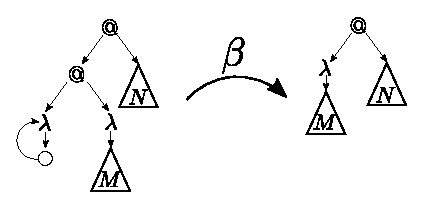
\includegraphics[width=1\linewidth]{../reduction2}
    \caption{test}
  \end{subfigure}

\end{figure}
\begin{figure}[htb]\ContinuedFloat
  \centering
  \begin{subfigure}{0.55\textwidth}
    \includegraphics[width=1\linewidth]{../reduction3}
    \caption{test}
  \end{subfigure}
  \caption{test}
\end{figure}
\clearpage 
  Powtarzając otrzymujemy więc \(\lambda\)-term w postaci normalnej. \qed

\end{dowod}
\begin{twierdzenie} 
  (\emph{Własność \(\mathrm{SN}_{\beta}\)}) Wszystkie \(\lambda\)-termy mają własność silnej normalizacji.
\end{twierdzenie}
\begin{itemize}
\item WCR: \(\forall a,\,b,\,c\in A\, (a\longrightarrow b \land a\longrightarrow c)\to \exists d\in A\,(b\longrightarrow^{*} d \land c\longrightarrow^{*} d)\)
\item CR: \(\forall a,\,b,\,c\in A\, (a\longrightarrow^{*} b \land a\longrightarrow^{*}c)\to \exists d\in A\,(b\longrightarrow^{*} d \land c\longrightarrow^{*} d)\)
\end{itemize}
\begin{twierdzenie} 
  \emph{(Lemat Newmana)} Niech \(\to\) bedzie relacją binarną spełniającą \(SN\). Jeśli \(\to\) spełnia WCR, to spełnia CR.
\end{twierdzenie}
\begin{dowod}
\end{dowod}

\begin{twierdzenie} 
  (\emph{Własność \(\mathrm{SN}_{\beta}\)}) Każdy \(\lambda\)-term w stylu Churcha własność silnej normalizacji.
\end{twierdzenie}
\begin{dowod}
\end{dowod}

